% !TEX program = lualatex
% !TEX encoding = UTF-8
\documentclass[paper=a4, fontsize=11pt]{jlreq}

% 必要なパッケージの読み込み
\usepackage{luatexja}
\usepackage{graphicx}
\usepackage{booktabs}
\usepackage{tabularx}
\usepackage{hyperref}
\usepackage{tikz}
\usetikzlibrary{shapes.geometric, arrows, positioning, fit, backgrounds}

\title{SportEase の情報の取り扱い}
\author{佐藤佑作} % 必要に応じて記入してください
\date{\today}

\begin{document}

\maketitle

\section{情報の取り扱い}
このアプリは Google アカウントでユーザー認証を行っている 。
高専のメールアドレスでのみログインできるように、ホワイトリストで制限している。

利用する  Google アカウント情報はGoogle メールアドレスのみである 。
\begin{itemize}
    \item  Google メールアドレス
\end{itemize}

使用用途は以下の通りである:

\begin{table}[h]
    \centering
    \caption{情報の使用用途}
    \begin{tabularx}{\textwidth}{|l|X|}
        \toprule
        情報 & 用途 \\
        \midrule
        メールアドレス & ユーザー認証、アプリ内でユーザーを一意に識別するためのID \\
        \bottomrule
    \end{tabularx}
\end{table}

\newpage

ユーザーの表示名に関しては、初回ログイン時に以下の画面で設定し、その後自由に変更可能にできる 。
\begin{figure}[htbp]
  \centering
  \includegraphics[width=0.8\linewidth]{./first-login.png}
  \caption{初回ログイン時の表示}
  \label{fig:image}
\end{figure}


\newpage

\section{外部設計}

\subsection{ユーザーロール}
本システムでは以下の3つのユーザーロールを定義し、権限管理を行っている。\\
必要に応じてロールを増やすことはできるが、権限管理はこの3つのベースロールで行っている。

\begin{table}[h]
    \centering
    \caption{ユーザーロール一覧}
    \begin{tabularx}{\textwidth}{|l| X|}
        \toprule
        ロール名 & 概要 \\
        \midrule
        Student (一般学生) & 主に情報の閲覧(対戦表、試合結果、クラスの進捗)および通知の受信を行う。  \\ \midrule
        Admin (行事委員) & イベント全体の管理、試合結果の入力・承認、スケジュールの変更、MVP投票の管理など、運営に必要な全機能にアクセス可能。 \\ \midrule
        Root (システム管理者) & システム設定、ホワイトリスト管理、マスターデータ(スポーツ、クラス等)の管理を行う最高権限。 \\
        \bottomrule
    \end{tabularx}
\end{table}

\subsection{機能要件}
各ロールにおける利用可能な機能の詳細は以下の通りである。

\subsubsection{Student (一般学生)}
一般的な学生ユーザーに割り当てられるロールであり、以下の機能を利用可能である。
\begin{itemize}
    \item \textbf{アカウント管理}:
    \begin{itemize}
        \item Googleアカウントを用いたログイン・ログアウト
        \item プロフィール設定(表示名、所属クラスの登録)
    \end{itemize}
    \item \textbf{情報閲覧}:
    \begin{itemize}
        \item 開催中のイベント情報の閲覧
        \item 各競技のトーナメント表・対戦組み合わせの閲覧
        \item 試合結果および勝敗のリアルタイム確認
        \item クラス別の総合得点・進捗状況・順位の閲覧
        \item 昼企画(リレー・綱引き等)の結果閲覧
    \end{itemize}
    \item \textbf{チーム管理(自クラスのみ)}:
    \begin{itemize}
        \item 所属クラスのチームメンバー編成機能(メンバーの追加・削除)
        \item チームメンバーの確認
    \end{itemize}
    \item \textbf{通知・その他}:
    \begin{itemize}
        \item 試合開始・結果等のWeb Push通知の受信
        \item MVP投票への参加(投票権がある場合)
    \end{itemize}
\end{itemize}

\subsubsection{Admin (行事委員)}
イベント運営の実務を担当するロールであり、Studentの全機能に加え、以下の管理機能を利用可能である。
\begin{itemize}
    \item \textbf{試合進行管理}:
    \begin{itemize}
        \item 試合開始時間の変更・調整
        \item 試合結果(スコア・勝者)の入力・確定
        \item 試合ステータスの更新(試合中、終了など)
        \item 昼企画(リレー・綱引き等)の予選・決勝結果の入力
    \end{itemize}
    \item \textbf{運営管理}:
    \begin{itemize}
        \item 前日・当日の出欠確認・登録
        \item 各競技の参加定員数の調整・変更
        \item ユーザーの表示名修正(不適切な名前の修正等)
        \item 運営用画像・PDF資料(要項・ルールブック等)のアップロード
        \item MVP投票状況の確認・集計
        \item 行事委員権限の付与・剥奪
    \end{itemize}
\end{itemize}

\subsubsection{Root (システム管理者)}
システムの全権限を持つロールであり、マスターデータの管理を含む以下の高度な機能を利用可能である。
\begin{itemize}
    \item \textbf{システム・イベント設定}:
    \begin{itemize}
        \item ログイン許可リスト(ホワイトリスト)の管理(追加・削除・一括インポート)
        \item 新規イベントの作成およびアクティブイベントの切り替え
        \item 雨天モード(スケジュール短縮・変更時)の切り替えおよび設定管理
    \end{itemize}
    \item \textbf{マスターデータ管理}:
    \begin{itemize}
        \item 競技種目の新規作成・削除
        \item クラス情報の管理および在籍学生数の登録(CSVインポート対応)
        \item 昼企画のグループ分け・テンプレート管理
        \item 全競技のトーナメント表の一括自動生成・プレビュー
    \end{itemize}
    \item \textbf{全体通知}:
    \begin{itemize}
        \item 全ユーザーまたは特定のロールに向けた任意のお知らせ通知の配信
    \end{itemize}
\end{itemize}

\subsection{画面構成・遷移}
本システムはWebブラウザ上で動作するSPA (Single Page Application) であり、以下の画面構成を持つ。

\begin{itemize}
    \item \textbf{ログイン画面}: Googleアカウントによる認証エントリポイント。
    \item \textbf{ダッシュボード (ホーム)}: ログイン後の初期画面。ユーザーロールに応じたメニューを表示。
    \item \textbf{学生向けメニュー (Student)}:
    \begin{itemize}
        \item \textbf{マイページ}: プロフィール設定、クラス情報確認
        \item \textbf{競技・イベント情報}: トーナメント表閲覧、競技詳細、点数一覧
        \item \textbf{昼企画}: 昼競技の結果確認
        \item \textbf{その他}: QRコード表示、通知確認、通知申請
    \end{itemize}
    \item \textbf{運営管理者メニュー (Admin)}:
    \begin{itemize}
        \item \textbf{試合管理}: 試合結果入力、トーナメント進行管理、昼競技結果入力
        \item \textbf{参加管理}: クラス・チーム編成管理、QRコード読み取り・参加確認、出席登録
        \item \textbf{運営設定}: ロール管理、競技詳細設定、MVP投票管理
    \end{itemize}
    \item \textbf{システム管理者メニュー (Root)}:
    \begin{itemize}
        \item \textbf{マスター管理}: イベント作成、競技種目設定、ホワイトリスト管理
        \item \textbf{全体設定}: 雨天モード設定、トーナメント一括生成、クラス人数設定
        \item \textbf{コンテンツ管理}: 競技要項アップロード、MVP確認
    \end{itemize}
\end{itemize}

\subsection{動作環境}
\begin{itemize}
    \item \textbf{クライアント端末}: スマートフォン(iOS/Android)、タブレット、PC
    \item \textbf{推奨ブラウザ}: Google Chrome, Safari, Microsoft Edge (各最新版)
    \item \textbf{ネットワーク}: インターネット接続必須(学内Wi-Fiまたはモバイルネットワーク)
\end{itemize}

\subsection{非機能要件}
\begin{itemize}
    \item \textbf{セキュリティ}:
    \begin{itemize}
        \item Google OAuth2 (OpenID Connect) による堅牢な認証
        \item 指定ドメイン (@sendai-nct.jp / .ac.jp) およびホワイトリストによるアクセス制限
        \item 常時SSL/TLS化 (HTTPS) による通信の暗号化
    \end{itemize}
    \item \textbf{パフォーマンス・可用性}:
    \begin{itemize}
        \item WebSocketを用いたリアルタイムな試合経過・結果の配信
        \item コンテナ技術 (Docker) による環境の一貫性と高い移植性
    \end{itemize}
\end{itemize}

\section{内部設計}

\subsection{システムアーキテクチャ}
本システムはDockerコンテナを用いたマイクロサービス構成を採用している。

\begin{itemize}
    \item \textbf{Reverse Proxy (Traefik)}: エントリーポイントとしてHTTPS通信の終端、Let's EncryptによるSSL証明書の自動更新、およびFrontend/Backendへのルーティングを行う。
    \item \textbf{Frontend (Frontapp)}: SvelteKit (Node.js) を用いたSSR/CSRハイブリッド構成。ユーザーインターフェースを提供。
    \item \textbf{Backend (Backapp)}: Go言語 (Gin Framework) によるREST APIサーバー。ビジネスロジックおよびWebSocketによるリアルタイム配信を担当。
    \item \textbf{Database (DB)}: MySQL 8.0。永続化データを管理。
\end{itemize}

\subsection{技術スタック}
\begin{table}[h]
    \centering
    \caption{採用技術一覧}
    \begin{tabularx}{\textwidth}{l l}
        \toprule
        カテゴリ & 技術 \\
        \midrule
        フロントエンド & SvelteKit, TailwindCSS, TypeScript \\
        バックエンド & Go 1.24, Gin, Gorilla WebSocket \\
        データベース & MySQL 8.0 \\
        インフラ & Docker, Docker Compose, Traefik v2 \\
        認証 & Google OAuth2 (OpenID Connect) \\
        \bottomrule
    \end{tabularx}
\end{table}

\subsection{データモデル設計}
主なエンティティとその役割は以下の通りである。

\begin{itemize}
    \item \textbf{Users}: ユーザーID、メールアドレス、ロール、表示名を管理。
    \item \textbf{Events}: 球技大会等のイベント単位。アクティブなイベントの設定が可能。
    \item \textbf{Sports / Classes}: 競技種目および参加クラスのマスターデータ。
    \item \textbf{Teams / Entries}: クラス・競技ごとのチーム編成およびエントリー情報。
    \item \textbf{Tournaments / Matches}: トーナメント構造および個々の試合データ(開始時刻、スコア、勝者)。
    \item \textbf{Notifications}: Web Push通知の購読情報および通知履歴。
\end{itemize}

\subsection{API設計}
RESTful APIを採用し、リソースごとにエンドポイントを定義している。
\begin{itemize}
    \item \texttt{/api/auth}: 認証関連(Googleログイン、プロファイル取得)
    \item \texttt{/api/events}: イベント情報の取得・更新
    \item \texttt{/api/admin}: 管理機能全般(試合結果更新、マスタ管理)
    \item \texttt{/api/student}: 学生向け読み取り専用API
    \item \texttt{/api/ws}: WebSocketエンドポイント(トーナメント表のリアルタイム更新等)
\end{itemize}

\subsection{ディレクトリ構成}
本システムの主要なソースコード構成は以下の通りである。

\begin{itemize}
    \item \texttt{frontapp/} (Frontend: SvelteKit)
    \begin{itemize}
        \item \texttt{src/routes/}: ページコンポーネントおよびSvelteKitのリ APIエンドポイント。
        \item \texttt{src/lib/}: 再利用可能なUIコンポーネント、ユーティリティ関数、ストア(状態管理)。
        \item \texttt{static/}: 静的ファイル(画像、フォント等)。
    \end{itemize}
    \item \texttt{backapp/} (Backend: Go)
    \begin{itemize}
        \item \texttt{cmd/}: アプリケーションのエントリーポイント (main.go)。
        \item \texttt{internal/router/}: Ginフレームワークを用いたルーティング定義。
        \item \texttt{internal/handler/}: HTTPリクエストを処理するビジネスロジック層。
        \item \texttt{internal/repository/}: データベース操作を抽象化するデータアクセス層。
        \item \texttt{internal/models/}: データベースのテーブル構造に対応するGo構造体定義。
        \item \texttt{db/migrations/}: データベースのスキーマ定義およびマイグレーション用SQLファイル。
    \end{itemize}
\end{itemize}

\subsection{データベース設計}
主要なテーブルとその役割は以下の通りである。

\begin{table}[h]
    \centering
    \caption{主要テーブル一覧}
    \begin{tabularx}{\textwidth}{|l|X|}
        \toprule
        テーブル名 & 概要 \\
        \midrule
        \texttt{users} & ユーザー情報(UUID, メールアドレス, 表示名, ロール等) \\ \midrule
        \texttt{classes} & クラス情報(クラス名, 学生数, イベントID) \\ \midrule
        \texttt{events} & イベント情報(大会名, 年度, 開催期間) \\ \midrule
        \texttt{sports} & 競技種目マスター(サッカー, バスケ等) \\ \midrule
        \texttt{teams} & クラス・競技ごとのチーム情報 \\ \midrule
        \texttt{matches} & 試合情報(トーナメント位置, 対戦チーム, スコア, 勝者) \\ \midrule
        \texttt{notifications} & Web Push通知の送信ログと内容 \\ \midrule
        \texttt{noon\_game\_*} & 昼企画(リレー等)に関連する設定・結果データ群 \\
        \bottomrule
    \end{tabularx}
\end{table}

\subsection{処理フロー例 (トーナメント進行)}
試合結果が入力され、トーナメント表が更新されるまでのデータフローは以下の通りである。

\begin{enumerate}
    \item \textbf{結果入力}: Adminユーザーが管理画面から試合のスコアを入力し、確定ボタンを押下する。
    \item \textbf{APIリクエスト}: フロントエンドから \texttt{POST /api/admin/match/result} が送信される。
    \item \textbf{バックエンド処理}:
    \begin{itemize}
        \item \texttt{matches} テーブルの該当レコード(スコア、勝者ID、ステータス)を更新する。
        \item 勝者が決定した場合、トーナメントの構造に基づき、次戦 (\texttt{next\_match\_id}) の対戦チームとして勝者を自動設定する。
        \item WebSocketを通じて、接続中の全クライアントに対して「試合更新イベント」をブロードキャストする。
    \end{itemize}
    \item \textbf{リアルタイム更新}:
    \begin{itemize}
        \item 各クライアント(Student/Admin画面)がWebSocketメッセージを受信する。
        \item トーナメント表コンポーネントが再レンダリングされ、リロードなしで最新の勝敗結果が反映される。
    \end{itemize}
\end{enumerate}

% 画像を挿入する場合は、画像ファイルをプロジェクト内に配置し、以下のコメントアウトを外してください。
\begin{figure}[h]
    \centering
    \resizebox{\textwidth}{!}{
    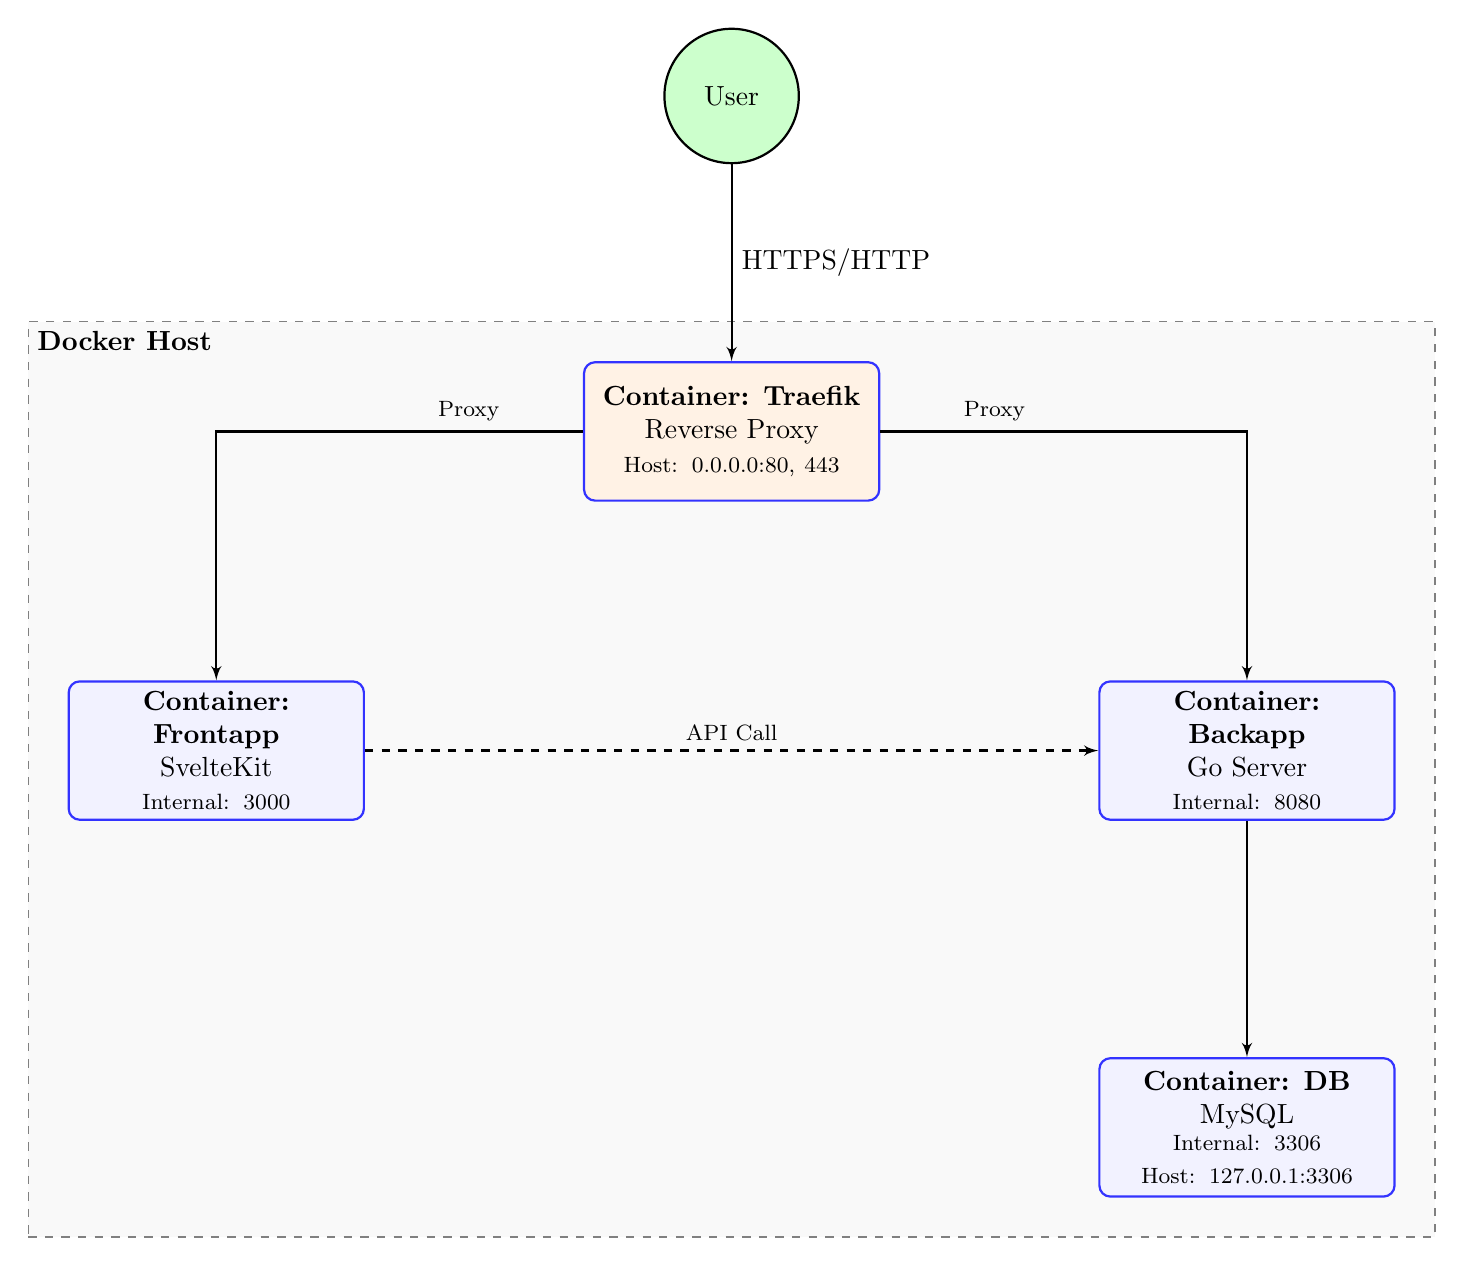
\begin{tikzpicture}[node distance=2.5cm, auto,
            % Styles
            container/.style={rectangle, draw=blue!80, fill=blue!5, thick, text width=10em, text centered, rounded corners, minimum height=5em},
            dbshape/.style={cylinder, cylinder uses custom fill, cylinder body fill=yellow!20, cylinder end fill=yellow!10, shape border rotate=90, aspect=0.25, draw=black, thick, text width=6em, text centered, minimum height=4em},
            user/.style={circle, draw=black, fill=green!20, thick, text width=4em, text centered},
            line/.style={draw, -latex', thick},
            dashedline/.style={draw, -latex', thick, dashed}
        ]

        % Nodes
        \node [user] (user) {User};

        % Traefik
        \node [container, below=of user, fill=orange!10] (traefik) {
            \textbf{Container: Traefik}\\
            Reverse Proxy\\
            \footnotesize{Host: 0.0.0.0:80, 443}
        };

        % Frontend
        \node [container, below left=of traefik, xshift=-1cm, yshift=-0.5cm] (frontend) {
            \textbf{Container: Frontapp}\\
            SvelteKit\\
            \footnotesize{Internal: 3000}
        };

        % Backend
        \node [container, below right=of traefik, xshift=1cm, yshift=-0.5cm] (backend) {
            \textbf{Container: Backapp}\\
            Go Server\\
            \footnotesize{Internal: 8080}
        };

        % Database
        \node [container, below=of backend, yshift=-0.5cm] (db) {
            \textbf{Container: DB}\\
            MySQL\\
            \footnotesize{Internal: 3306}\\
            \footnotesize{Host: 127.0.0.1:3306}
        };

        % Edges
        \path [line] (user) -- node[right] {HTTPS/HTTP} (traefik);
        \path [line] (traefik) -| node[pos=0.1, above left, font=\footnotesize] {Proxy} (frontend);
        \path [line] (traefik) -| node[pos=0.1, above right, font=\footnotesize] {Proxy} (backend);
        \path [dashedline] (frontend) -- node[above, font=\footnotesize] {API Call} (backend);
        \path [line] (backend) -- (db);

        % Docker Host Box
        \begin{scope}[on background layer]
            \node [draw=black!50, dashed, fill=gray!5, fit=(traefik) (frontend) (backend) (db), inner sep=0.5cm, label={[anchor=north west]north west:\textbf{Docker Host}}] (host) {};
        \end{scope}

    \end{tikzpicture}
    }
    \caption{システム構成図(Dockerコンテナ構成)}
\end{figure}



\end{document}